%!TEX root = ../../main.tex
\chapter{STCF 11}
\label{stcf11}

\lhead{Chapitre ??. \emph{Chapter Title Here}}

\section{Présentation de la configuration standard 11}
\label{sec:presentation_stcf11}

La configuration standard 11~\cite{Fransson:1999uq}
est une aube de stator de turbine oscillant sur 
son premier mode de flexion à régimes: un subsonique et un
transsonique. Le premier mode est 

\begin{table}[htbp]
  \ra{1.3} \centering
  \begin{tabular}{lccc}
    \toprule
    \phantom{abdefghijk}& $C_t$ & $C_p$ & $\eta$ \\
    \midrule
    Take-off & $-1.448$ & $2.895$ & $0.565$ \\
    Cruise & $-1.067$ & $5.32$ & $0.789$ \\
    \bottomrule
  \end{tabular}
  \caption{Point de fonctionnement.}
  \label{tab:flight_condition}
\end{table} 

\begin{itemize}
  \item un régime subsonique où l'écoulement
        ne présente pas de phénomènes physiques majeurs.
        Ce cas permet de facilement valider le code numérique
        avant de l'éprouver sur un point de fonctionnement plus
        complexe,
  \item un régime transsonique qui se distingue par la 
        présence d'un 
        choc à environ $75\%$ de la corde axiale,
        et d'un bulbe de décollement à $\approx 30\%$
        de la corde axiale.
        Ce cas permet, quant à lui, d'évaluer la robustesse
        du code dans le cas d'un écoulement complexe.
\end{itemize}

La cascade d'aubes est placée dans un canal annulaire fixe de l'École
Polytechnique Fédérale Lausanne~Fig.\ref{fig:canal_annulaire}.
Ce dernier permet d'obtenir un écoulement tant transsonique que subsonique
grâce à la forme de sa veine d'essai. De plus, le canal étant fixe,
l'instrumentation des pales est relativement aisée.
La vibration des pales est assurée par un actuateur électromagnétique
permettant la mise en place d'une onde tournante de type mode à diamètre.

\begin{figure}[htbp]
  \centering
  \includegraphics*[width=0.40\textwidth]{./ANNULAR_CHANNEL.pdf}
  \caption{Canal annulaire}
  \label{fig:canal_annulaire}
\end{figure}


\section{Instrumentation de l'aube}

L'instrumentation est réalisée sur la peau d'une des aubes.
Des sondes de pressions statiques non intrusives permettent
de mesurer la répartition de cette dernière 
le long de la corde axiale. Étant donné le caractère instationnaire
des phénomènes aéroélastiques, l'acquisition temporelle de la pression
statique est réalisée afin de donner les résultats sous forme de partie imaginaire
et réelle du premier harmonique de pression.

Pour la mise en valeur des effets stationnaires, le nombre de Mach isentropique est 
calculé à partir des mesures de pression statique. Ce dernier est défini par
% 
\begin{equation}
  M_{is} = \sqrt{\left[\left(\frac{P_{i0}}{P_s}\right)^{\frac{\gamma - 1}{\gamma}} - 1 \right] \cdot \frac{2}{\gamma -1}},
  \label{eq:mach_isentropique}
\end{equation}
% 
où $P_{i0}$ est la pression totale de référence et $P_s$ la pression statique
mesurée sur la peau de l'aube. Cette dernière évolue le long de la corde axiale.
Étant donné que $P_{i0}$ est constant, le nombre de Mach isentropique va suivre une
évolution similaire à l'inverse de la pression statique, ainsi il peut être
décrit comme l'interprétation de la pression statique sous forme de vitesse
adimensionnée, lorsque la pression totale n'est pas facilement accessible. En effet,
les aubes sont facilement instrumentées par des capteurs de pression statique, car ils 
ne nécessitent pas d'être intrusifs. Ceci est lié à la conservation de la
pression statique ($\frac{\partial P}{\partial n} = 0$ sous hypothèses de Prandtl). En revanche,
les prises de pression totale nécessitent de créer un arrêt isentropique, ce qui 
entraînerait la mise en place de sondes intrusives et de surcroît hors de la surface de
la peau de la pale.

Pour l'évaluation des effets aéroélastiques, des mesures de l'amplitude $\widetilde{Cp}$ et de la
phase $\widetilde{\phi}$ du premier harmonique de pression sont données sous forme de répartition
le long de la corde du profil définies par
% 
\begin{equation}
  \begin{split}
    C_{p, inst} &= \frac{c \cdot \widetilde{P_s}(x)}{h \cdot (P_{i0} - P_{s0})}, \\
    \widetilde{Cp} &= |C_{p, inst}|, \\
    \widetilde{\phi} &= \textrm{arg}(C_{p, inst}),
  \end{split}
  \label{eq:cp_inst}
\end{equation}
% 
où $\widetilde{P_s}(x)$ est l'évolution sur la corde du premier harmonique de pression
et $P_{s0}$ est la pression statique en entrée du canal.

La géométrie, les résultats expérimentaux et les articles associés à la 
configuration standard $11$ sont disponibles sur internet~\cite{STCF11_url}.
Des études sont présentes dans la littérature, principalement pour le cas 
transsonique de par la complexité de l'écoulement qui s'y développe 
\cite{Cinnella:2004fk, Sbardella:2001fk, Duta:2002uq, Campobasso:2003fk}.
Ces derniers montre l'adéquation des résultats numériques avec ceux expérimentaux, 
ce qui en fait un cas test intéressant.

\section{Paramètres numériques}

Le calcul est réalisé avec le code de calcul \textit{elsA}. Un schéma décentré de type
Roe du troisième ordre est choisi. Pour la modélisation de la turbulence, 
le modèle de Spalart-Allmaras est utilisé. Afin de pouvoir comparer les résultats obtenus
avec une approche de référence, les calculs instationnaires sont réalisés avec l'approche
classique dite de pas de temps dual.

L'aube de turbine est maillée en suivant une topologie O4H. Le nombre de points est de 160
autour de l'aube et les $y^+$ calculés sont $\mathcal{O}(1)$, ce qui correspond à l'état de 
l'art pour un tel calcul.

\section{Résultats stationnaires}

\subsection{cas subsonique}

Le cas subsonique est représentatif d'une turbine fonctionnant au point nominal.
L'écoulement ne présente pas de phénomènes particuliers~Fig.~\ref{fig:stcf11_rans_2D_subsonic}.
La répartition de nombre de Mach isentropique est 

\begin{figure}[htbp]
  \centering
  \includegraphics*[width=0.45\textwidth]{STCF11_SUBSONIC_FIELD_MIS_BW.png}
  \caption{Champ stationnaire}
  \label{fig:stcf11_rans_2D_subsonic}
\end{figure}

\begin{figure}[htbp]
  \centering
  \includegraphics*[width=0.45\textwidth]{STCF11_RANS_SUBSONIC.pdf}
  \caption{Répartition du nombre de Mach isentropique fonction de la corde axiale}
  \label{fig:stcf11_rans_mis_subsonic}
\end{figure}



\subsection{cas transsonique}

\begin{figure}[htbp]
  \centering
  \includegraphics*[width=0.45\textwidth]{STCF11_TRANSONIC_FIELD_MIS_BW.png}
  \caption{Champ stationnaire}
  \label{fig:stcf11_rans_2D_transonic}
\end{figure}

\section{Résultats instationaires}

\subsection{cas subsonique}

\subsection{cas transsonique}



% 
% Pour les simulations numériques, 
% 
% Les paramètres numériques utilisés pour les simulations suivantes sont rappelés ci-dessous:
% \begin{itemize}
%   \item schéma spatial de Roe d'ordre 3,
%   \item modèle de turbulence de type $k-l$ de Smith.
% \end{itemize}
% 
% \paragraph{Cartographie de champ 2D}
% 
% Les cartographies de champ 2D sont donnés en figure \ref{fig:stcf11_rans_2D}. La pression statique est représentée en contours et les lignes de courant en traits fins, ou en d'autres termes, la trajectoire que suit le fluide. Le cas subsonique ,\fig \ref{fig:stcf11_rans_2D_subsonic}, ne présente pas de singularité, le fluide accélère sur l'extrados et décélère sur l'intrados de la pale. En revanche, le cas transsonique présente de fortes singularités qui expliquent son étude à des fins de validation. En effet, ce dernier présente deux phénomènes aérodynamiques complexes repérés dans la figure \ref{fig:stcf11_rans_2D_transonic}. 
% \begin{itemize}
%   \item \textit{zone I}: bulle de décrochage. Avant que le profil décroche (c'est à dire que les lignes de courant ne suivent plus le profil), une bulle de décrochage peut se former. Or cette non-linéarité va réagir avec les vibrations de la pale comme nous le verrons plus tard.
%   \item \textit{zone II}: cette zone présente un choc. C'est un phénomène dimensionnant dans une turbomachine. On peut le visualiser par la discontinuité en pression qu'il présente.
% \end{itemize}
% 
% 
% \paragraph{Comparaison avec les résultats expérimentaux}
% Comme rappelé dans la section \ref{sec:presentation_stcf11}, des résultats stationnaires expérimentaux sont donnés sur le site internet du KTH. La comparaison avec les présents résultats est reportée en figure \ref{fig:stcf11_rans_expe}.
% 
% Ces résultats montrent la bonne adéquation entre l'expérience et les calculs numériques. Les principales disparités observées sont similaires à celle rencontrées dans la littérature:
% \begin{itemize}
%     \item cas subsonique: surestimation du Mach isentropique sur l'extrados de la configuration lors de la recompression,
%     \item cas transsonique: sous estimation de l'intensité du choc sur l'extrados et surestimation de la position du choc (zone II détaillé précédemment), même si les disparités dans les mesures expérimentales mettent en avant leurs incertitudes.
% \end{itemize}
% 
% 
% 
% \begin{figure}[H]
%     \center
%     \subfigure[cas subsonique]{ 
%       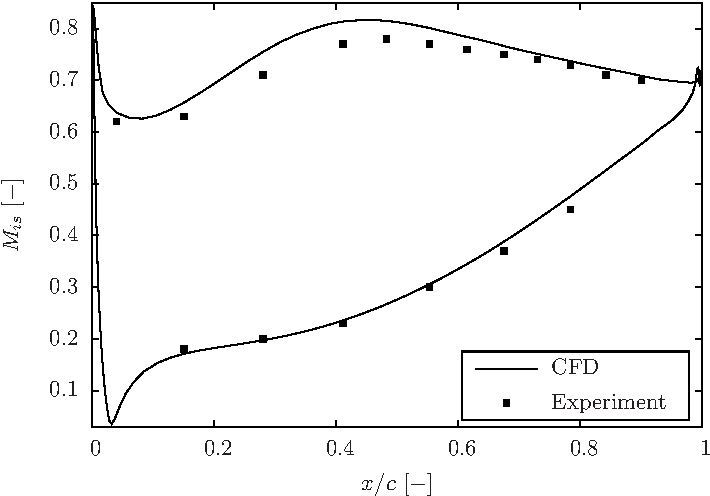
\includegraphics[width=7.5cm]{IMAGES/STCF11_RANS_SUBSONIC.pdf}}
%     \subfigure[cas transsonique]{ 
%       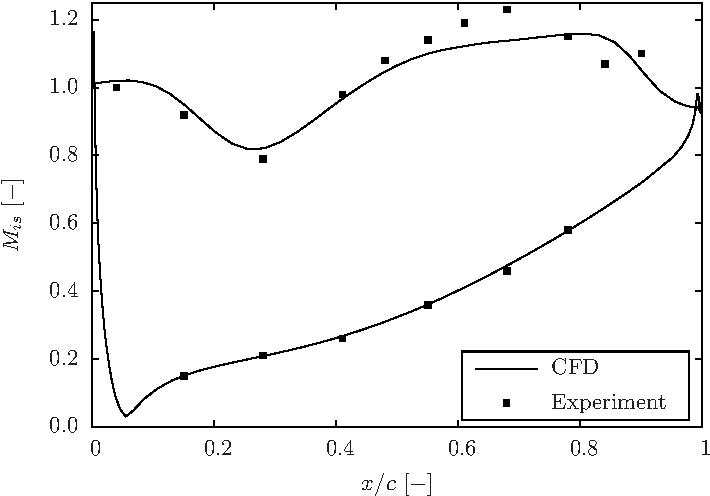
\includegraphics[width=7.5cm]{IMAGES/STCF11_RANS_TRANSONIC.pdf}}
%     \caption{Résultats stationnaires}
%     \label{fig:stcf11_rans_expe}
% \end{figure}
% 
% \section{Résultats aéroélastiques}
% 
% Des premiers résultats aéroélastiques ont été obtenus avec le code de calcul \elsa. La fréquence du mode imposé est $211.6 Hz$ et l'amplitude de $0.0035$.
% Les résultats sont donnés en terme d'évolution de l'amplitude et de la phase du premier harmonique de pression sur la pale. La figure \ref{fig:stcf11_ael} montre les résultats obtenus avec \elsa avec une approche DTS et HBT. Les résultats sont comparés à l'expérience et aux résultats de Cinnella et al. (voir Réf. \cite{Cinnella:2004fk}). En effet, les résultats numériques obtenus par ces derniers sont téléchargeables sur internet \footnote{http://cemec.poliba.it/BENCHMARK\_SC11.txt}, ce qui permet une comparaison supplémentaire.
% 
% L'analyse de ces résultats permet de dire que:
% \begin{itemize}
%   \item la prédiction des paramètres conditionnant l'amortissement est bonne que ce soit en DTS ou en HBT. Rien ne permet de qualifier l'une ou l'autre de meilleure. Ainsi, l'approche HBT pour prédire le flottement est validée,
%   \item les régions qui "pulsent" (comprendre où l'amplitude du coefficient de pression augmente) semble être les régions où il y a des phénomènes physiques importants. En effet, la région du bulbe de décrochage ($0 \leq x/c \leq 0.3$, zone I présentée dans la partie précédente) et la région du choc ($0.7 \leq x/c \leq 0.9$, zone II) ont toutes les deux un pic de coefficient de pression.
% \end{itemize}
% 
% 


% Fransson et al.:
% 
% - veine annulaire non tournante cascade de EPF-Lausanne
% - 20 pales excitée électromagnitiquement et contrôller pour vibrer en mode tournant
% - les suspensions des pales sont contruites afin de reproduire la fréquence propre
% et la direction du mode de flexion de la pale entrain de faire un movement rigide
% - STCF 11: choc droit à 75\% de la pale sur l'extrados
% - différences dans l'amortissement du à de petites différences dans la région du choc
% - mesures de pression totale et statique dans les plans e1 et e2 ainsi que derrière la cascade
% - les mesure pariétales sont faites au moyen de "pressure-taps" pour le cas stationnaires et de
% "miniaturized piezo-resistive pressure transducer" pour le cas instationnaire, embarqué à mi-hauteur de pale,
% sur différentes pales
% - en changeant un peu les conditions, le choc peut varier de 5\% en position
% - raisons de variations entre les expé et le numérique: effets du fluide réel non
% capté par les méthodes numérique ou perdu à cause des techniques de mesure (effet 3D, 
% couche limite des murs (hub/shroud), erreurs sur les relevés de pression, estimation des angles 
% du fluide, moyennage des grandeurs en azimuth et en hauteur radial)
% - amortissement varie énormement en fonction des conditions amonts
% dans le cas transsonique (fig 4.)
% - en revanche on a des tendances dans les mesures locales 
% - c'est la position du choc qui est la première source d'incertitude

% Cinnella et al.:
% 
% - pour les différents IBPA, elle multiplie le nb de canaux:
% np=z*360deg/IBPA, où z est l'entier minimum qui donne une valeur
% entière de np
% - présentation du cas STCF 11: conditions d'entrée (Mach et angle de l'écoulement)
% et reynolds de 1,2.10+6 basé sur la longueur de la corde et les conditions amonts
% - remise en cause de l'expé lorsque les bars de confiance à 95 \% sont de l'ordre
% de la valeur moyenne du point, gros écart lorsque Fransson et al. modifient les
% conditions amonts -> on regarde les résultats locaux

% Campobasso et Giles:
% 
% - ils font du LUR, couplage faible avec une méthode GMRES pour stabiliser
% les oscillations qu'ils obtiennent dans les champs stationnaires.
% - en fait ces oscillations sont dues à la physique du pb (décollement,
% vortex shedding ...)
% - ils imposent l'IBPA comme un déphasage complexe (comme nous)
% - ils calculent le travail du fluide sur la structure (donc pas les
% courbes d'amortissement de Fransson directement)

% Duta et al.:
% 
% - belle intro sur l'utilité de l'aéroélasticité
% - biblio sur méthodes de couplage faible
% - place du LUR dans simu aéroélastiques
% - LUR: hypothèse périodicité et petites perturbations
% - calcul adjoint pour estimer la réponse forcée de différents
% type de distortions amonts
% - si le sillage impacte la pale de manière uniforme, la réponse forcée sera maximale,
% si on a un déphasage du moment de l'impacte: déphasage=> minimisation
% du travail du fluide sur la structure

% Sbardella et Imregun
% 
% - papier de ref sur l'AEL
% - calculs 3D AEL bien mais les designers ont besoin de calculs qui tournent vite
% - le flottement est généralement un phénomène qui apparait dans des conditions off-design
% - sur prédiction sur le cas subsonique à mi-corde, mais raison de cet effet
% discuter dans Fransson et al.
% - nombre de Mach pré-choc est très sensible aux conditions d'entrée pour le 
% cas transsonique (fransson et al.), d'où les différences avec les essais
% - il vaut mieux que la turbulence ne soit pas gelée
% - rapport 30 sur le temps de calcul

% Fransson: Annular cascade experiments
% 
% - avantages de la veine d'essai annulaire non tournante:
%       * pas de murs latéral dans la direction circonférentielle => pas de réflexion des ondes de pression
%       * écoulement périodique dans le domaine
%       * instrumentation facile car pas de rotation
%       * écoulement supersonic possible grâce à la forme du tube d'écoulement
% - peut accueillir 20 pales
% - les pales sont en vibration forcée par le biais d'un exciteur électromagnétique
% la vibration des pales est mesurée par des capteurs de déplacement inductifs.
% ces capteurs sont fixés sur un anneau d'impact. Ce dernier est controllé axialement
% par un système hydraulique. Cela permet de limiter la vibration des pales si elles 
% commencent à osciller en flottement naturel (auto-déclanché) afin de ne pas casser
% les amortisseurs. Un système électronique de contrôle permet d'établir et de maintenir un 
% mode de vibration organisé de la cascade.
% - les frequences d'excitations doivent être proches de la fréquence propre 
% du système pale-mass-ressort